% !TEX encoding = UTF-8
% !TEX TS-program = pdflatex
% !TEX root = ../Tesi.tex
% !TEX spellcheck = en-EN

%************************************************
\chapter{Discrete Element Method}
\label{cap:dem}
%************************************************

The discrete element method (\acs{DEM}) is derived from Molecular Dynamics. \\ 
For each particle $i$ inside the domain, a \acs{DEM} code
follows the trajectory and calculates the force that particle $i$ exerts on
particle $j$.
The main forces involved are: gravity, contact forces due to collisions, and
further interactions such as electrostatic, Van der Waals, cohesive forces and fluid-solid interactions in 
multiphase flows. \\
Two approaches can be implemented for this method:
\begin{itemize}
  \item{hard spheres,}
  \item{soft spheres.}
\end{itemize} 
The hard-sphere approach is well-suited for binary collisions, easy to
calculate, but cannot predict multi-particle interactions.
It is mainly used for dilute flows, rather then in the dense flows we
investigated.

%\section{DEM}
%\label{sec:dem}
% \section{Hard spheres approach}
% \label{sec:hardspheresapproach}
% \info{words on hard spheres approach}

\section{Soft sphere approach}
\label{sec:softspheresapproach}

\info{could use tikz for this image}
\begin{figure}[!h]
\centering
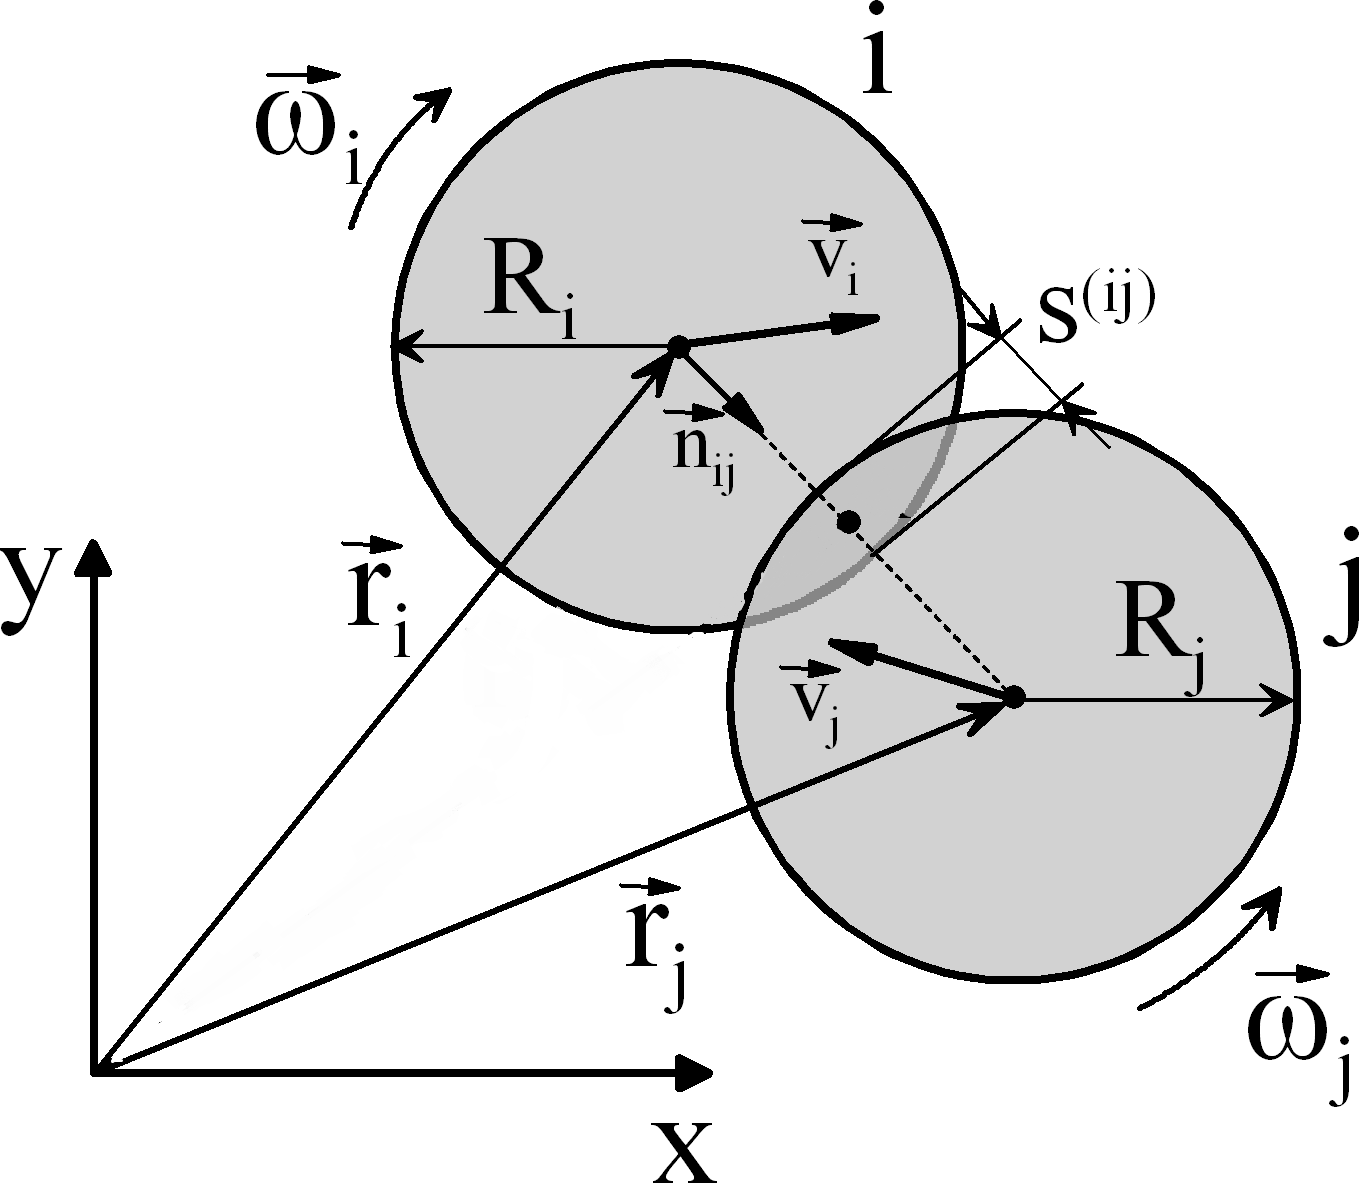
\includegraphics[width=.6\columnwidth]{images/109twospheres}
\caption[Two spheres]{Two colliding spheres with the soft-sphere approach.}
\label{fig:109twospheres}
\end{figure}
The soft sphere approach considers the deformation of particles when they
collide with each other. From the vector in Fig. \ref{fig:109twospheres} we can
define after time \textit{t} the normal and tangential overlaps \acs{xin} and
\acs{xit}:
\begin{equation}
\xi_n = R_i + R_j - \mathbf{n} \cdot (\mathbf{r}_j - \mathbf{r}_i),
 \label{eq:xin}
\end{equation}

\begin{equation}
\xi_t = \int_{0}^{t}{\mathit{dt'}|\mathbf{v}_t(\mathit{t'})|} ,
 \label{eq:xit}
\end{equation}

where the subscript \acs{n} stands for normal and \acs{t} for tangential. 
At this point we can divide the contact models into:
\begin{itemize}
  \item{linear, e.g. Hooke,}
  \item{non-linear, e.g. Hertz.}
\end{itemize}

\subsection{Hertz}
\label{subsec:hertz}

For the raw material used in this work 
Di Renzo and Di Maio \cite{RefWorks:145} suggested using the non-linear
Hertzian model without cohesion for the particle-particle and particle-wall contacts. 
For an elasto-perfectly-plastic-viscous model the contact forces, normal and
tangential, are:
\begin{equation}
\mathbf{F}_{n} = k_n \xi_n \mathbf{n} + \gamma_n \mathbf{v}_n , 
\label{eq:fn}
\end{equation}

\begin{equation}
\mathbf{F}_t = 
 \begin{cases}
k_t \xi_t \mathbf{t} + C_t \mathbf{v}_t  & \text{if } |k_t \xi_t \mathbf{t} +
C_t \mathbf{v}_t| \leq \mu_s |\mathbf{F}_n| ,\\
\mathbf{t} \mu_s |\mathbf{F}_n|  & \text{else.}
\end{cases}
 \label{eq:ft}
\end{equation}
%************************************************
The Coulomb's law of friction is the condition in the tangential force
formulation.\\
Here, \acs{k} and \acs{gamma} are respectively the stiffness and damping
coefficients, while \textbf{v} is the velocity.
Both the normal and the tangential
force comprise two terms, a spring force and a damping force. 
The tangential (or shear) force is a ``history'' effect that accounts for the
tangential displacement (``tangential overlap'') between the particles for the
duration of contact.
The \acs{kn}, \acs{kt}, \acs{gamman}, and \acs{gammat} coefficients are
calculated from the material properties as follows:
%************************************************
\begin{equation}
\begin{aligned}
	k_n &= \frac{4}{3} E_{eq} \sqrt{R_{eq} \xi_n} ,\\
	\gamma_n &= 2 \sqrt{\frac{5}{6}} \beta \sqrt{S_n m_{eq}} ,\\
	k_t &= 8 G_{eq} \sqrt{R_{eq}} \xi_n ,\\
	\gamma_t &= 2 \sqrt{\frac{5}{6}} \beta \sqrt{S_t m_{eq}} .
\end{aligned}
\label{eq:hertz}
\end{equation}

%************************************************
In addition to the equations \ref{eq:hertz} the following relations (Eqns. \ref{eq:equivProp2}) are required:
%************************************************
\begin{equation}
\begin{aligned}
 \frac{1}{E_{eq}} & = \frac{1-\nu_i^2}{E_i} + \frac{1-\nu_j^2}{E_j} ,\\
 \frac{1}{G_{eq}} & = \frac{2(2+\nu_i)(1-\nu_i)}{E_i} + \frac{2(2+\nu_j)(1-\nu_j)}{E_j} ,\\
 \frac{1}{R_{eq}} &= \frac{1}{R_i} + \frac{1}{R_j} ,\\
 \frac{1}{m_{eq}} &= \frac{1}{m_i} + \frac{1}{m_j} ,\\
 \beta & = \frac{\ln(e)}{\sqrt{ln^2(e)+\pi^2}} ,\\
 S_n & = 2 E_{eq} \sqrt{R_{eq} \delta_n} ,\\
 S_t & = 8 G_{eq} \sqrt{R_{eq} \delta_n} ,\\
 k_r & = k_t R_{eq}^2 .\\
\end{aligned}
\label{eq:equivProp2}
\end{equation}


%************************************************

The coefficient of sliding friction \acs{mus} is 
one of the particle-based \acs{DEM} parameter we investigated, 
another being the coefficient of rolling friction (\acs{mur}),
that can be simulated with these models:
\begin{itemize}
  \item{constant direct torque (CDT),}
  \item{elasto-plastic-spring-dashpot.}
\end{itemize}

In the paper by Wensrich and Katterfeld \cite{RefWorks:87}, further details on
the method can be found.\\

% \subsection{Hooke}
% \label{subsec:hooke}


%This granular model uses the following formula for the contact force between
% two granular particles (Eq. \ref{eq:forceij}):
% %************************************************
% \begin{equation}
 F_{ij} = 
\begin{cases}
F_{n,ij} + F_{t,ij} = \left( k_n \delta_{n,ij} + \gamma_n v_{n,ij} \right) + \left( k_t \delta_{t,ij} + \gamma_t v_{t,ij} \right) & \text{if } r < d ,\\
0    & \text{if } r > d ,\\
\end{cases}
 \label{eq:forceij}
\end{equation}

% %************************************************


% , $r$ is the
% distance between two particles of radii $R_i$ and $R_j$, and $d = R_i + R_j $ is
% % the contact distance.
% 
% 
% 
% 
% In the contact law we used, 
% the tangential component of the contact force between two generic particles
% ($F_t$) is truncated to fulfil:
% % %************************************************
% % \begin{equation}
F_{t,ij} \leq \mu_s F_{n,ij},
 \label{eq:force_t}
\end{equation}

% % %************************************************
% 
% where $F_n$ is the normal component and 

\subsection{Elasto-plastic-spring-dashpot 2}
\label{subsec:epsd2}

For coarse non-spherical particles, \acs{mur} is a critical parameter and describes
inter-particle friction in medium to dense granular flow simulations. 
It is proportional to the 
torque counteracting the rotation of the particle. 
The \acs{mur} parameter enters the 
equations according to the elasto-rolling resistance model presented by Wensrich and 
Katterfeld \cite{RefWorks:87} and Ai et al. \cite{RefWorks:131} 
based on the work of Jiang et al. \cite{RefWorks:143}. 
A scheme of the particles interaction can be seen in Fig.
\ref{fig:128springdashpot}.\\
\begin{figure}[!htb]
\centering
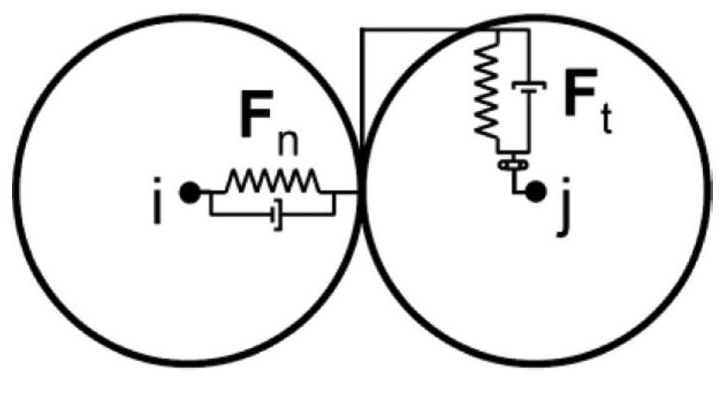
\includegraphics[width=.40\columnwidth]{images/128springdashpot}
\caption[Spring dashpot]{Spring dashpot model.}
\label{fig:128springdashpot}
\end{figure}
The model is called EPSD2 in \acs{LIGGGHTS} and is appropriate for both one-way and cyclical rolling cases.
The maximum magnitude of rolling resistance torque is (Eq. \ref{eq:trmax}):

%************************************************
\begin{equation}
T_{r~max} = \mu_r R_r |\tilde{F_n}| ~,
 \label{eq:trmax}
\end{equation}

%************************************************

where $R_r$ is the equivalent radius and $F_n$ the normal force.
The last two particle-based \acs{DEM} parameters we investigated were 
the particle density (\acs{rhop})
and the coefficient of restitution (\acs{CoR}) as defined by
\citet{RefWorks:131}.
Together with the others they are listed in Table \ref{tab:08DEMparameters}.\\

\begin{table}[h]
\centering
\begin{tabular}{l}
\hline 
    Radius \ac{R} (m)   \\ [5pt]

	Size distribution (-) \\ [5pt]

    Young's modulus \ac{E} (Pa)  \\ [5pt]

    Poisson's ratio \ac{nu} (-) \\ 
     Time step \ac{deltat} (s) \\ [5pt]
        \hline
     Coefficient of sliding friction \ac{mus} (-)\\  [5pt]
    Coefficient of rolling friction \ac{mur} (-) \\ [5pt]
    Coefficient of restitution \ac{CoR} (-)   \\ [5pt]
     Particle density $\ac{rhop} = \frac{mass ~ of ~ one ~ particle}{volume ~ of
     ~ one ~ particle}$ ($kg/m^3$)  \\ [5pt]
     Geometry factor \ac{dCylDp} (-)  \\ [5pt]
   
\hline
\end{tabular}
\caption[DEM parameters]{DEM parameters. The upper parameters were
identical in all simulations. The lower parameters were constant in each
simulation, but were varied between simulations.}
\label{tab:08DEMparameters}
\end{table}



\section{Literature Values}
\label{sec:literaturevalues}

There are yet ways to determine contact parameters directly by measuring
material properties or by performing particle based experiments, see e.g.
\citet{RefWorks:177}, \citet{RefWorks:181}, and \citet{RefWorks:186}.
\citet{RefWorks:140} and \citet{RefWorks:190}
are two of the most prominent examples of parameters identification by
theoretical analysis. 

\subsection{Limitations}
\label{subsec:limitations}

The available literature data, however, focused on glass spheres, while
non-sphericity was one of the fields we wanted to investigate. 
Further, it is related to all the microscopic parameters we analysed. 
Also the procedure of \citet{RefWorks:177}, although on
industrial samples (aluminium oxide), still had mostly spherical particles. 
In addition, these methodologies are laborious, 
since they have to be performed for every new granular material prior to a $DEM$
simulations. 
Especially for the already cited rolling friction parameter, it is arduous to
link the rolling friction parameter to the non-sphericity of the particle. 


\section{Unresolved CFD-DEM}
\label{sec:unresolvedcfddem}
%************************************************

The existence of particles immersed in a fluid influences its behaviour. 
Keeping aside the short-scale flow field, the local averages inside the
Navier-Stokes fluid equations could account for the particles.
This is called the \textit{unresolved \acs{CFD}-\acs{DEM} approach}, and can be
seen in Fig. \ref{fig:130unresolvedcfddem}.\\
\begin{figure}[!htb]
\centering
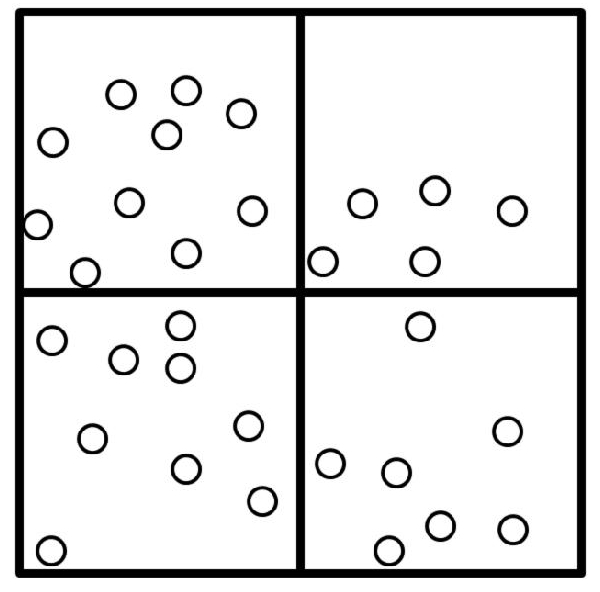
\includegraphics[width=.40\columnwidth]{images/130unresolvedcfddem}
\caption[Unresolved CFD-DEM]{Unresolved CFD-DEM \cite{Refworks:202}.}
\label{fig:130unresolvedcfddem}
\end{figure}
On the hypothesis of having \textit{g(r)} a convenient averaging
function, which is non-negative, smooth, asymptotically zero for large $r$, normalized, \citet{Refworks:201}
defines the local void fraction ($\varepsilon(\mathbf{r},t)$), the volume of the
fluid ($V_f(t)$) over the total volume, as:
\begin{equation}
\varepsilon(\mathbf{r},t) = \int_{V_f(t)}{d^3 r' g(|\mathbf{r} - \mathbf{r'}|)}.
 \label{eq:voidfraction}
\end{equation}

We define local mean values of fluid point properties as:
\begin{equation}
\bar{a}(\mathbf{r},t) = \frac{1}{\varepsilon(\mathbf{r},t)} \int_{V_f(t)}{d^3 r'
g(|\mathbf{r} - \mathbf{r'}|) a(\mathbf{r'},t)},
 \label{eq:a}
\end{equation}

which came from a slowly varying a rapidly fluctuating part:
\begin{equation}
\label{eq:a2}
a(\mathbf{r},t) = \bar{a}(\mathbf{r'},t) + a'(\mathbf{r},t).
\end{equation}

Particle properties, on the solid volume $V_s(t)$ and the solid fraction
$\phi(\mathbf{r},t)$, are expressed as field quantities as:
\begin{equation}
\begin{align*}
\bar{b}(\mathbf{r},t) &= \frac{1}{\phi(\mathbf{r},t)} \int_{V_f(t)}{
g(|\mathbf{r} - \mathbf{r'}|) b(\mathbf{r'},t) \dd^3 r'} \\
& \approx
\frac{1}{\phi(\mathbf{r},t)} \sum_{p}{g(\mathbf{r} - \mathbf{r}_p)
V_p b_p(t)}.
\end{align*}
 \label{eq:b}
\end{equation}

The approximation is valid when $g(r)$ varies slowly over the particles length
scale, and the averages of the derivatives can be written as:
\begin{equation}
\begin{align*}
\nabla_{\mathbf{r}} \varepsilon (\mathbf{r},t) \bar{a}(\mathbf{r},t) 
&=
\int_{V_f(t)}{
a(\mathbf{r'}, t) \nabla_{\mathbf{r}} g(|\mathbf{r} - \mathbf{r'}| )  \dd^3 r'} \\
&=
- \int_{S_f(t)}{ a(\mathbf{S},t) g(|\mathbf{r} - \mathbf{S}|) \dd \mathbf{S} + 
\varepsilon (\mathbf{r},t) \overline{\nabla a}(\mathbf{r},t)} \\
& \approx
\sum_{p}{\int_{S_p(t)}{ a(\mathbf{S},t) g(|\mathbf{r} - \mathbf{S}|)  \dd
\mathbf{S}}} + \varepsilon (\mathbf{r},t) \overline{\nabla a}(\mathbf{r},t).
\end{align*}
 \label{eq:divepsa}
\end{equation}

Further, for time derivatives we can write:
\begin{equation}
\begin{align*}
\frac{\partial}{\partial t}\varepsilon (\mathbf{r},t) \bar{a}(\mathbf{r},t) 
&=
\int_{V_f(t)}{
\frac{\partial a(\mathbf{r'}, t)}{\partial t} g(|\mathbf{r}
- \mathbf{r'}| )  \dd^3 r'} \\
&+ \lim \frac{1}{\Delta t} \left[
\int_{V_f(t + \Delta t)}{ a(\mathbf{r'}, t) g(|\mathbf{r} - \mathbf{S}|)  \dd^3
r'} - \int_{V_f(t)}{ a(\mathbf{r'}, t) g(|\mathbf{r} - \mathbf{S}|)  \dd^3 r'}
\right ]\\
& \approx
\varepsilon (\mathbf{r},t) \overline{\dot{a}}(\mathbf{r},t) - 
\sum_{p}{\int_{S_p(t)}{\mathbf{v_s} a(\mathbf{S},t) g(|\mathbf{r} - \mathbf{S}|) 
\dd \mathbf{S}}}.
\end{align*}
 \label{eq:ddtepsa}
\end{equation}

We could now write in Eq. \ref{eq:divepsa} $a = \rho \mathbf{u}$, so it becomes:
\begin{equation}
\nabla_{\mathbf{r}} \varepsilon (\mathbf{r},t) \overline{\rho \mathbf{u}}(\mathbf{r},t) 
 \approx
\sum_{p}{\int_{S_p(t)}{ \rho \mathbf{u}(\mathbf{S},t) g(|\mathbf{r} - \mathbf{S}|)  \dd
\mathbf{S}}} + \varepsilon (\mathbf{r},t) \overline{\nabla {\rho
\mathbf{u}}}(\mathbf{r},t).
 \label{eq:divepsrhou}
\end{equation}

Similarly, for Eq. \ref{eq:ddtepsa}, we consider $a = \rho$, and we write:
\begin{equation}
\frac{\partial}{\partial t}\varepsilon (\mathbf{r},t) \bar{\rho}(\mathbf{r},t) 
\approx
\varepsilon (\mathbf{r},t) \overline{\dot{\rho}}(\mathbf{r},t) - 
\sum_{p}{\int_{S_p(t)}{\mathbf{v_s} \rho(\mathbf{S},t) g(|\mathbf{r} - \mathbf{S}|) 
\dd \mathbf{S}}}.
 \label{eq:ddtepsrho}
\end{equation}

At this point, it is easy to demonstrate that by merging Eq. \ref{eq:divepsrhou}
and Eq. \ref{eq:ddtepsrho} we obtain the \textit{volume-averaged continuity
equation}:
\begin{equation}
\frac{\partial}{\partial t}\varepsilon (\mathbf{r},t) \overline{\rho}(\mathbf{r},t) +
\nabla \cdot \varepsilon (\mathbf{r},t) \overline{\rho
\mathbf{u}}(\mathbf{r},t)  = 0.
 \label{eq:continuity}
\end{equation}

In case of incompressible flow, Eq. \ref{eq:continuity} becomes:
\begin{equation}
\frac{\partial}{\partial t}\varepsilon (\mathbf{r},t)  +
\nabla \cdot \varepsilon (\mathbf{r},t) \overline{
\mathbf{u}}(\mathbf{r},t)  = 0.
 \label{eq:continuityincompressible}
\end{equation}

In the same way, for the Navier-Stokes momentum equation:
\begin{equation}
\int_{V_f(t)}{\left[g(|\mathbf{r} - \mathbf{r'}|) \rho_f \left(\frac{\partial
\mathbf{u}}{\partial t} + ( \mathbf{u} \cdot \nabla) \mathbf{u} \right) \right]
\dd^3 r'} = 
\int_{V_f(t)}{\left[g(|\mathbf{r} - \mathbf{r'}|) \nabla \cdot \tau +
\rho_f \mathbf{g} \right] \dd^3 r'} ,
 \label{eq:nsmomentumequation}
\end{equation}

which can be written:
\begin{equation}
\rho_f \varepsilon (\mathbf{r}, t) \left(\frac{\partial
\mathbf{\overline{u}}}{\partial t} + ( \mathbf{\overline{u}} \cdot \nabla)
\mathbf{\overline{u}} \right) = 
\nabla \cdot (\overline{\tau} - \overline{R}) -\sum_{p}{g(|\mathbf{r} -
\mathbf{r_p}|)\mathbf{F}_{p-f}(\mathbf{\overline{u}}, \varepsilon,
\mathbf{v}_p, d_p) + \rho_f \varepsilon (\mathbf{r}, t) \mathbf{g}} ,
 \label{eq:nsmomentumequation2}
\end{equation}

where:
\begin{equation}
\overline{R}(\mathbf{r}) = 
\rho_f 
\int_{V_f(t)}{g(|\mathbf{r} - \mathbf{r'}|)  
\mathbf{u'}(\mathbf{r'}, t) \circ \mathbf{u'}(\mathbf{r'}, t)
\dd^3 r'} .
 \label{eq:rr}
\end{equation}

To complete the system, we add the particles equation of motion:
\begin{equation}
m_p \frac{\partial \mathbf{v}_p}{\partial t} = 
\mathbf{F}_{p-f}(\mathbf{\overline{u}}, \varepsilon,
\mathbf{v}_p, d_p) + m_p \mathbf{g} + \Phi_{p-p}(\mathbf{r}_p, \{\mathbf{r}_k
\}),
\label{equ:equationofmotion}
\end{equation}

where $\Phi_{p-p}$ is a force field, which acts on particle $p$ because of the
remaining particles.
This \textit{unresolved \acs{CFD}-\acs{DEM} approach} works as long as the exact
trajectories of each particle can be negliged.\\
For completeness, we could say that also the equation of motion can be averaged
over space, obtaining:
\begin{equation}
\frac{\partial}{\partial t}\phi (\mathbf{r},t) \rho_p (\mathbf{r},t) +
\nabla \cdot \phi (\mathbf{r},t) \overline{\rho_p
\mathbf{v}_p}(\mathbf{r},t)  = 0.
 \label{eq:eomaveraged}
\end{equation}

If the spheres have the same density, we can write:
\begin{equation}
\frac{\partial}{\partial t}\phi (\mathbf{r},t) +
\nabla \cdot \phi (\mathbf{r},t) \overline{
\mathbf{v}_p}(\mathbf{r},t)  = 0,
 \label{eq:eomaveraged2}
\end{equation}

Finally:
\begin{equation}
\begin{align*}
\rho_p \phi (\mathbf{r}, t) \left(\frac{\partial
\mathbf{\overline{v}}_p}{\partial t} + ( \mathbf{\overline{v}}_p \cdot \nabla)
\mathbf{\overline{v}}_p \right) 
& = 
\sum_{p}{g(|\mathbf{r} - \mathbf{r_p}|)\Phi_{p-p}}
- \nabla \cdot S \\ 
& + \sum_{p}{g(|\mathbf{r} - \mathbf{r_p}|)\mathbf{F}_{p-f}} 
+ \phi(\mathbf{r}, t) \rho_p \mathbf{g} ,
\end{align*}
 \label{eq:eom3}
\end{equation}

where:
\begin{equation}
S(\mathbf{r}) = 
\sum_{p}{m_p g(|\mathbf{r} - \mathbf{r}_p|)  
\mathbf{v'}_p \circ \mathbf{v'}_p} .
 \label{eq:sr}
\end{equation}

The main advantage of this model is to allow a greater number of particles to be
considered, since they are treated as an additional averaged fluid: this is
called the \textit{two-fluid model}.
Hovewer, this model work poorly in a dense system like our, see
\citet{Refworks:202}, and was thus not considered further.
